% Template for QoMEX'12 paper; to be used with:
%          spconf.sty  - ICASSP/ICIP LaTeX style file, and
%          IEEEbib.bst - IEEE bibliography style file.
% --------------------------------------------------------------------------
\documentclass{article}
\usepackage{spconf,amsmath,epsfig}
\usepackage[utf8]{inputenc}
\usepackage{graphicx}
% autoref command
\usepackage[pdftex,urlcolor=black,colorlinks=true,linkcolor=black,citecolor=black]{hyperref}
\def\sectionautorefname{Section}
\def\subsectionautorefname{Subsection}
\def\figureautorefname{Fig.}
\def\subfigureautorefname{Fig.}

% Example definitions.
% --------------------
\def\x{{\mathbf x}}
\def\L{{\cal L}}

% Title.
% ------
\title{DEFINING AESTHETIC PRINCIPLES FOR AUTOMATIC MEDIA GALLERY LAYOUT\\
FOR VISUAL AND AUDIAL EVENT SUMMARIZATION BASED ON SOCIAL NETWORKS}
%
% Two addresses (uncomment and modify for two-address case).
% ----------------------------------------------------------
\twoauthors
  {Thomas Steiner$^1$, Ruben Verborgh$^2$}
	{$^1$Universitat Politècnica de Catalunya\\
	Llenguatges i Sistemes Informàtics (LSI)\\
	08034 Barcelona, Spain\\
	\texttt{tsteiner@lsi.upc.edu},\\
	\texttt{gabarro@lsi.upc.edu}}
  	{Joaquim Gabarro$^1$, Rik Van de Walle$^2$}
	{$^2$Ghent University -- IBBT,\\
	ELIS -- Multimedia Lab,\\
	B-9050 Ledeberg-Ghent, Belgium\\
	\texttt{ruben.verborgh@ugent.be},\\
	\texttt{rik.vandewalle@ugent.be}}
%
\begin{document}
%\ninept
%
\maketitle
%
\begin{abstract}
In this paper, we define and discuss aesthetic principles
for the automatic generation of media galleries
based on media items retrieved from social networks
that---after a ranking and pruning step---can serve to authentically
summarize events and their atmosphere from a visual
and from an audial standpoint. 
\end{abstract}
%
\begin{keywords}
event summarization, media galleries, social networks,
media item ranking, media layout, aesthetics
\end{keywords}
%
\section{Introduction}
Mobile devices such as smartphones, together with social networks,
enable people to create, share, and consume media items
like videos or images.
They accompany their owners almost everywhere they go
and are thus omnipresent at all sorts of events.
Given a~stable network connection, event-related media items
and microposts are published on social networks
during events and afterwards.
Ranked media items stemming from multiple social networks
can serve to create authentic media galleries
that illustrate events and their atmosphere.
A~key feature for this task is the semantic enrichment
of media items and associated microposts
and the extraction of \textbf{visual}, \textbf{audial},
\textbf{textual}, \textbf{social}, and \textbf{aesthetic} features.

\begin{figure}[htb]
\centering
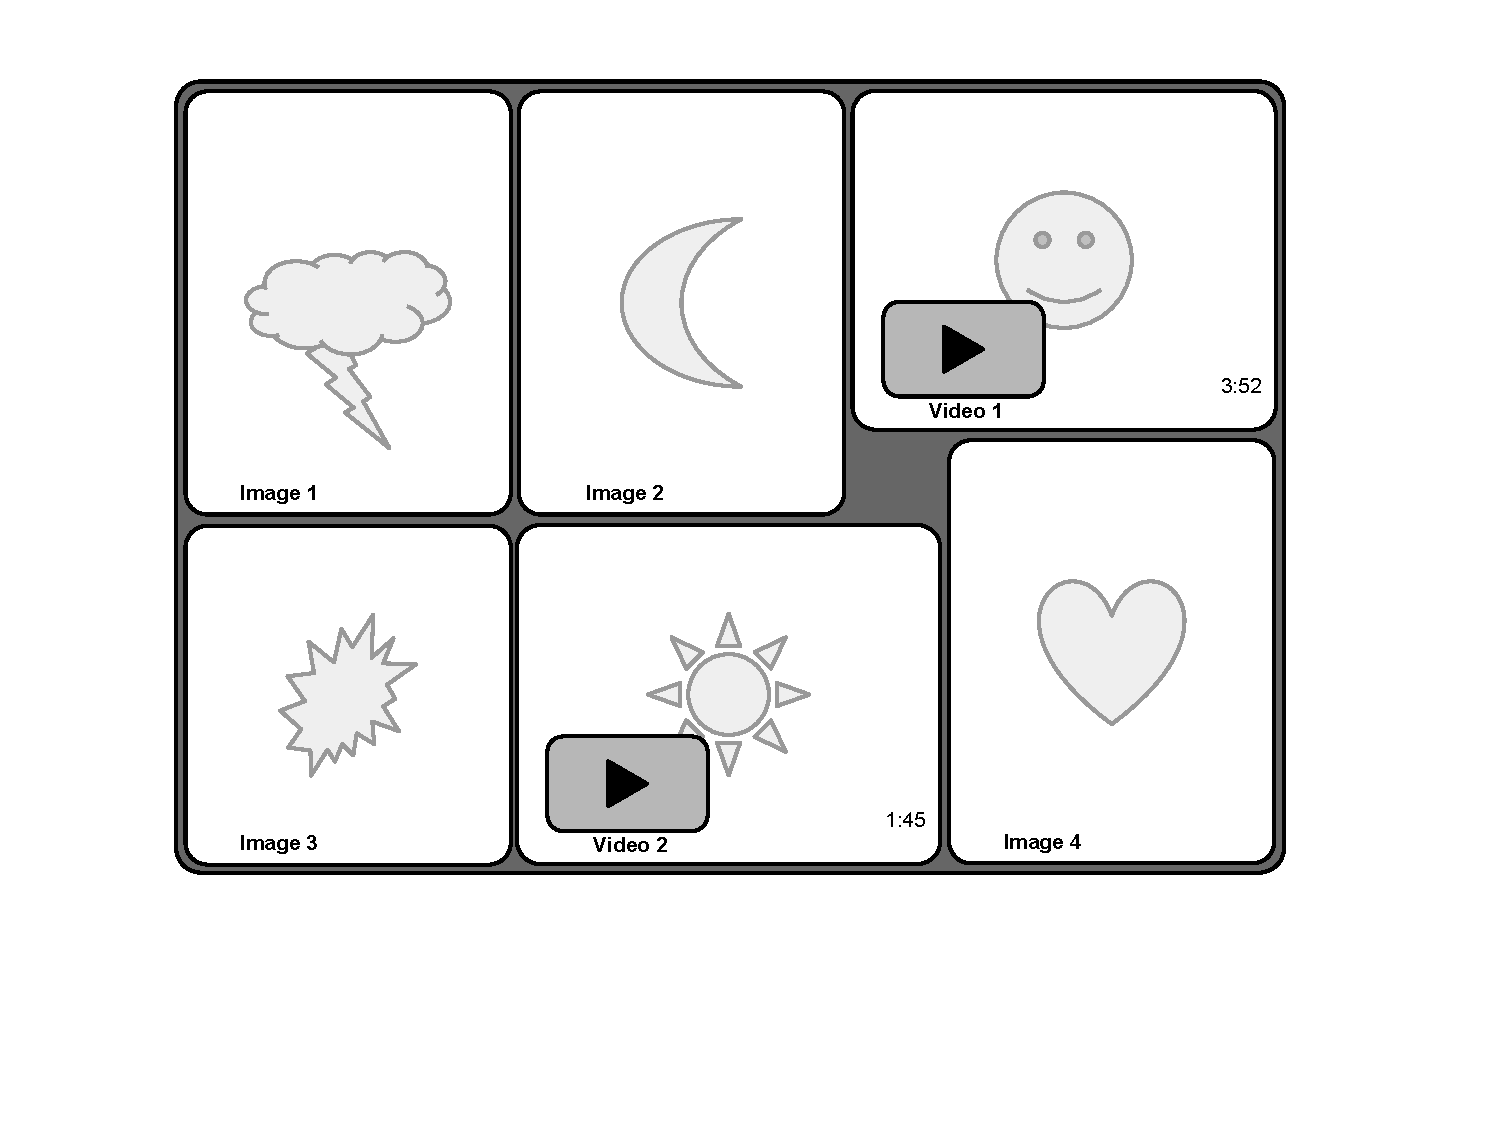
\includegraphics[trim=20mm 40mm 20mm 10mm, clip, width=0.75\columnwidth]{media-gallery.pdf}
\caption{Schematic media gallery with 5 images and 2 videos.}
\label{fig:media-gallery}
\end{figure}

\section{Related Work}
While enormous efforts have been made to extract those features
from media items and microposts on social networks in \emph{isolation},
to the best knowledge of the authors, remarkably less efforts 
can be detected for the extraction and the application
of \emph{all} those features in \emph{combination}
for \emph{all} types of media items including microposts.
In~\cite{Photo2011}, Sandhaus \emph{et al.} consider visual and
aesthetic features for the automatic creation of photo books.
Obrador \emph{et al.} use visual and aesthetic features
for a category-based approach to automatically assess
the aesthetic appeal of photographs~\cite{Photo2012}.
In~\cite{Playlist2006}, Knees \emph{et al.} use audial and textual
features for the automatic generation of music playlists.
Choudhury \emph{et al.} show in \cite{Sports2011} how social and textual
features can be used to achieve precise detection results 
of named entities and significant events in sports-related microposts.
In~\cite{YouTube2010}, Davidson \emph{et al.} show how visual,
textual, and social features can be used for personalized video recommendations.
A service called Storify~\cite{Storify2011} lets users manually combine
microposts, images, videos, and other elements onto one page for the purpose
of storytelling or summarizing an event,
and share stories permanently on the Web.
Finally, social networks present images and videos
often in grid-like galleries, sometimes resized
based on the amount of comments\footnote{http://twitpic.com/904yka/full}.

\section{Media Item Ranking Criteria}
In this section, we describe several feature categories that can serve to rank
media items retrieved from social networks. 
We assume (and are working on) media item extractors that,
given event-related search terms,
extract raw binary media items and associated microposts
from multiple social networks.

\noindent \textbf{Visual}
This category regards the actual contents of images and videos.
We distinguish \emph{low-level} and \emph{high-level} visual ranking criteria.
Examples for high-level ranking criteria are logo detection,
face recognition, or the separation in camera shots.
Examples for low-level ranking criteria are file size, pixel resolution,
video duration, geolocation, timestamp, etc.
Through optical character recognition,
text in media items can be converted to a textual feature.

\noindent \textbf{Audial}
This category regards the audio track of videos.
\emph{High-level} ranking criteria are the presence or absence
of silence, music, speech, or a mixture of the prior.
Similar to visual features before,
audial \emph{low-level}  features are the average bit rate,
whether the audio is overdriven, volume, etc.
Through audio-transcription, speech can be converted to a textual feature.

\noindent \textbf{Textual}
This category regards the microposts that accompany media items.
Typically, microposts provide a~description of media items.
Using named entity disambiguation tools,
textual content can be linked to LOD cloud concepts~\cite{Facebook2011}.

\noindent \textbf{Social}
This category regards social network effects like shares, mentions,
number of views, expressions of (dis)likes, user diversity, etc.
Our previous work allows us to not only examine these effects
on a~\emph{single} social network (\emph{e.g.}, ReTweets on Twitter),
but in a~\emph{network-agnostic} way across multiple social networks.

\noindent \textbf{Aesthetic}
This category regards the desired outcome after the ranking, \emph{i.e.},
the media gallery that illustrates an event and its atmosphere.
Studies exist for the aesthetics of
automatic photo book layout~\cite{Photo2011},
photo aesthetics \emph{per se}~\cite{Photo2012},
video and music playlist generation~\cite{YouTube2010,Playlist2006},
however media gallery composition requires mixing video
\emph{and} image media items.

\section{Media Gallery Aesthetics}

\subsection{Definition}
A media gallery in our context is a compilation of images or videos
retrieved from social networks that are related to a given event.
Given a set $M = \{m_1,..., m_n\}$ of media items related to a certain event $e$,
and given a ranking formula $f$,
the set $M^\prime$ is the subset $M^\prime \subset M$
resulting after the application of $f$ to $M$: $f(M)=M^\prime$.
Each media item $m_i$ can either be an instance of video or image.
For each point $t_j$ on a timeline $T$, the state of the media gallery
at $t_j$ is defined for each media item $m_i$
as a set $S_j$ of $n$ tuples $s_{j,i}$, where
$s_{j,i}=\langle left, top, width, height, alpha, z-index, playing,
volume, start, animation \rangle$.
The properties follow the definitions of CSS, the $animation$ property
allows for the definition of CSS transitions
and transformations as defined in~\cite{CSSTransitions2009,CSSTransforms2012},
the $start$ property defines the start time in a video. 
A schematic media gallery at $t_j$ can be seen in \autoref{fig:media-gallery}.

\subsection{Audial Aesthetics}

\subsection{Visual Aesthetics}

\section{Future Work and Conclusion}

% References should be produced using the bibtex program from suitable
% BiBTeX files (here: strings, refs, manuals). The IEEEbib.bst bibliography
% style file from IEEE produces unsorted bibliography list.
% -------------------------------------------------------------------------
\bibliographystyle{IEEEbib}
\bibliography{steiner.bib}

\end{document}
